\section{Side investigation: fixing a small number of contradictions}\label{sec:repair}

Whichever reference is used, somebody has to find the repairs: the planetary stage for a repaired reference, unified's steering for a superposed one. This section asks how many contradictions a shift really creates, where they can be fixed, and whether the fixes lie in the space unified already searches. It combines theory with measurements on vanilla Space Age.

\subsection{Setup of the measurements}

The measurements ran in an isolated copy of the mod, which was stopped right after the planetary code had run (so no unified randomization), with the user's current startup settings and seeds 1--8. For each seed there are three scenarios: the raw ocean swap, the raw resource swap, and both. ``Raw'' means the swaps are applied by the mod's own \code{oceans.apply} and \code{resources.apply} with that seed's assignment, but \emph{without} scaffolds, recipe edits or extra patches. Each scenario records:
\begin{enumerate}[nosep]
\item the contradictions $D$: \code{check.required_failures} of the shifted game against vanilla, i.e.\ exactly PLANETCHECK's three rules;
\item the \emph{causes} of each contradiction: the feature pebbles that its vanilla witness (\code{top.path}) uses and that the shifted world lacks;
\item staged repair sorts (Section~\ref{sec:staged}) over ingredient slots, with repairs read off the witness and pruned with real sorts to an irreducible set;
\item the superposed graph $\Gsup$: whether it loses anything against the transported goals, and which debt edges its solvency-first witness needs.
\end{enumerate}
The code is in Appendix~\ref{app:experiment}. Everything is logic-level: it answers what the logic graph says is reachable, which is the project's source of truth.

\subsection{Contradictions are counted in the wrong unit}

\begin{table}[t]
\centering\footnotesize
\setlength{\tabcolsep}{3.2pt}
\begin{tabular}{@{}r rrrrr rrrrr rrrrr@{}}
\toprule
 & \multicolumn{5}{c}{ocean swap} & \multicolumn{5}{c}{resource swap} & \multicolumn{5}{c}{both} \\
\cmidrule(lr){2-6}\cmidrule(lr){7-11}\cmidrule(l){12-16}
seed & goals & causes & rep. & in & debt & goals & causes & rep. & in & debt & goals & causes & rep. & in & debt \\
\midrule
1 & 151 & 4 & 10 & 3 & 4 & 24 & 3 & 5 & 3 & 3 & 164 & 8 & 12 & 4 & 6 \\
2 & 151 & 4 & 10 & 3 & 4 & 139 & 3 & 5 & 4 & 3 & 76 & 8 & 13 & 6 & 6 \\
3 & 151 & 4 & 10 & 3 & 4 & 24 & 3 & 10$^{\dagger}$ & 10 & 3 & 166 & 8 & 11$^{\dagger}$ & 7 & 7 \\
4 & 151 & 4 & 10 & 3 & 4 & 51 & 3 & 5 & 4 & 3 & 164 & 8 & 13 & 6 & 6 \\
5 & 151 & 4 & 10 & 3 & 4 & 51 & 4 & 12$^{\dagger}$ & 12 & 4 & 166 & 9 & 15$^{\dagger}$ & 9 & 8 \\
6 & 151 & 4 & 10 & 3 & 4 & 139 & 2 & 3 & 3 & 2 & 76 & 7 & 11 & 5 & 5 \\
7 & 151 & 4 & 10 & 3 & 4 & 139 & 4 & 12$^{\dagger}$ & 12 & 4 & 166 & 9 & 14$^{\dagger}$ & 9 & 8 \\
8 & 151 & 4 & 10 & 3 & 4 & 139 & 4 & 8 & 6 & 4 & 76 & 9 & 15 & 7 & 7 \\
\bottomrule
\end{tabular}
\caption{Contradictions of raw shifts, seeds 1--8. \emph{goals}: failing goal pebbles (PLANETCHECK's rules). \emph{causes}: distinct lost feature pebbles on their vanilla witnesses. \emph{rep.}: irreducible root-first repair set (ingredient slots). \emph{in}: how many of those unified's recipe-ingredients handler may randomize. \emph{debt}: debt edges on the superposition's solvency-first witness, i.e.\ what settling by addition would take. $\dagger$: some goals are not reachable with \emph{any} ingredient repair (Section~\ref{sec:where}); the repair set covers the others.}
\label{tab:counts}
\end{table}


Table~\ref{tab:counts} gives the first answer. A raw shift creates many failing goal pebbles, \CountsFailRange\ per seed across the scenarios. These are not independent problems. They collapse to a handful of \emph{causes}, the lost features themselves (\CountsCauseRange), and to a similarly small number of \emph{repairs}. One cause fails many goals at once: when Aquilo loses its ammoniacal ocean, cryogenic science is lost in every room where it was automatable, together with everything that needs it.

So ``fixing a small number of contradictions'' is the right framing, as long as contradictions are counted at the cause or repair level. Counted by goal pebbles, the planetary check's own unit, the problem looks one to two orders of magnitude bigger than it is.

\begin{figure}[t]
\centering
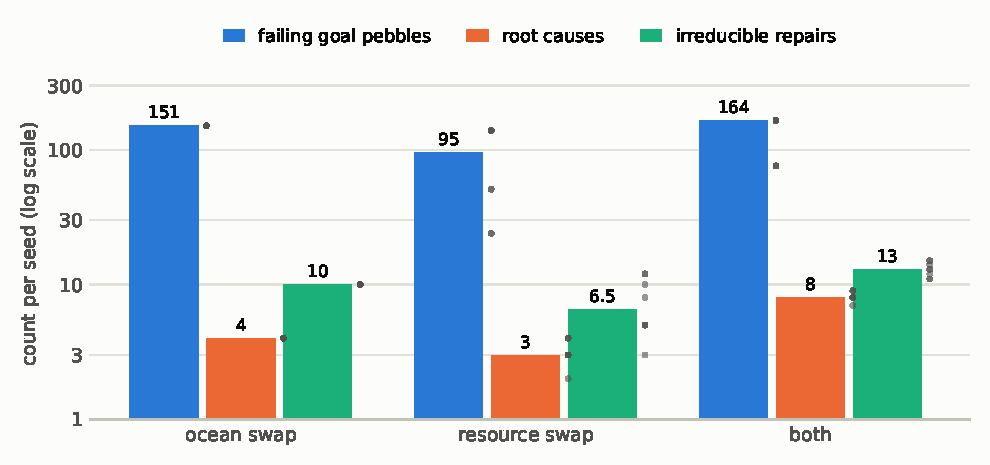
\includegraphics[width=\linewidth]{figs/counts.pdf}
\caption{Goal failures, root causes and irreducible repairs per scenario (median over seeds 1--8, bars; per-seed values, dots; log scale). A raw ocean swap fails around 150 goal pebbles, which trace back to four lost oceans and are fixed by about ten slot repairs.}
\label{fig:counts}
\end{figure}

\subsection{Repairs as relaxations}\label{sec:relax}

A repair changes what fills a slot. For the question \emph{where} a repair is needed, the filler does not matter yet, which suggests treating an opened slot as filled by ``anything available''.

\begin{definition}[Relaxed repair]
For a set $A$ of ingredient slots, $G\ominus A$ removes the in-edges of $A$ (the recipe no longer needs those ingredients). $A$ is a \emph{relaxed repair} if $\Goals_1\subseteq\Reach(G_1\ominus A)$.
\end{definition}

\begin{proposition}[Relaxation bound]\label{prop:relax}
If a goal is not in $\Reach(G_1\ominus K)$ for a class $K$ of slots, then no way of refilling the slots in $K$ reaches it.
\end{proposition}
\begin{proof}
Any refilling $G'$ is $G_1\ominus K$ plus one in-edge per slot, and those edges end in $\AND$ nodes (recipes). By Lemma~\ref{lem:monotone}, $\Reach(G')\subseteq\Reach(G_1\ominus K)$.
\end{proof}

A relaxed repair is monotone in $A$: opening more slots only reaches more. That makes it the right object for search. The \emph{minimum} relaxed repair is still NP-hard, by reduction from set cover: give each set its own slot, which opens an $\AND$ node that is otherwise unreachable, and make each element a goal $\OR$ node fed by the $\AND$ nodes of the sets containing it. In practice the instances are tiny, so greedy pruning to an \emph{irreducible} set (no single repair can be dropped) is enough.

Relaxation is also what separates the three kinds of fix:
\begin{itemize}[nosep]
\item a \textbf{scaffold variant} is the relaxation made real. The original recipe stays and a copy with a different filler is added, so nothing that used the original loses anything (monotone, like $G\ominus A$);
\item a \textbf{repair edit} realizes the relaxation by changing the recipe in place, which is only possible when one filler works in every context the recipe must keep (Section~\ref{sec:conflict});
\item a \textbf{leaf repair} opens slots far from the cause, in the consumers of what was lost.
\end{itemize}

\subsection{Staged sorts: witnesses that repair only where needed}\label{sec:staged}

The earliest-provider witness of a random sort does not care whether it uses an opened slot or the original ingredient. On a fully relaxed graph it therefore patches every consumer it meets: a first version of this experiment, which removed every unified-randomizable slot at once, reported 44 ``must-change'' slots on 22 recipes for seed~1's ocean swap. The fix is to make repairs \emph{come later in the sort} than everything that needs no repair.

\begin{definition}[Staged sort]
Replace each relaxable slot $m\to r$ of class $k$ by $m\to h\to r$ with an $\OR$ head $h$, and add an edge $\mathit{gate}_k\to h$, where $\mathit{gate}_k$ is an $\OR$ node with no inputs, so it starts closed. Sort. Then, for $k=1,2,\dots$, connect a source to $\mathit{gate}_k$ and \emph{continue the same sort} (\code{top.sort}'s cached mode with one new connection).
\end{definition}

\begin{proposition}[Properties of a staged sort]\label{prop:staged}
\leavevmode
\begin{enumerate}[nosep,label=(\alph*)]
\item After stage $k$, the reached pebbles are exactly $\Reach(G_1\ominus(\text{classes}\le k))$;
\item every pebble first reached in stage $s$ ranks after every pebble of earlier stages;
\item the earliest-provider witness of a goal first reached in stage $s$ opens no gate of a later class. It goes through a class-$s$ gate at a head only if the gate's pebble there ranks before the original ingredient's;
\item the gates on a witness form a relaxed repair.
\end{enumerate}
\end{proposition}
\begin{proof}
(a) The continuation processes every consequence of the new connection until nothing new is open, so it reaches the least model of the extended program (Lemma~\ref{lem:monotone}). (b) New pebbles are appended. (c) Witness pebbles have lower ranks than the pebble they back, so by (b) they belong to stage $s$ or earlier. (d) The witness is a derivation that uses only original edges and those gates (Lemma~\ref{lem:justification}).
\end{proof}

A staged sort ranks repair classes lexicographically: first see what needs no repair, then what needs only cheap repairs, and only then what needs expensive ones. With classes ordered by how undesirable a repair is, it is the practical form of a \emph{minimal-repair witness} for this logic. It is a heuristic, not an optimum, because earliest-provider witnesses do not minimize the number of gates. The solvency-first witness of Section~\ref{sec:constructions} is the same construction with the debt edges behind the gate. Figure~\ref{fig:staged} shows the mechanism.

\paragraph{Cost.} In the measurements, with the machine under heavy load from other runs, the medians over the 24 runs were: about 4\,s to rebuild the logic and sort it, 8\,s for a three-stage staged sort, 4\,s for the superposition's staged sort, and 46\,s for pruning (one full sort per candidate repair; 35--111\,s). Without pruning, a staged sort plus one verifying sort costs about three plain sorts, which is in line with the roughly four sorts today's scaffold selection takes. The group-halving pruning that \file{scaffolds.lua} already uses (\code{prune_groups}) would cut most of the rest.

\begin{figure}[t]
\centering
\begin{tikzpicture}[x=1cm,y=1cm]
\begin{scope}[on background layer]
\fill[cvan!7] (0,-0.35) rectangle (5.2,0.35);
\fill[crep!9] (5.2,-0.35) rectangle (8.9,0.35);
\fill[cshift!9] (8.9,-0.35) rectangle (12.6,0.35);
\end{scope}
\draw[-{Stealth}, thick, cgrey] (0,0) -- (13.2,0) node[right, lbl] {rank};
\node[lbl, anchor=south] at (2.6,0.4) {stage 0: no repairs};
\node[lbl, anchor=south] at (7.05,0.4) {stage 1: root slots open};
\node[lbl, anchor=south] at (10.75,0.4) {stage 2: other slots open};
\foreach \x in {0.6,1.4,2.3,3.1,4.0,4.7}{\node[pebble, fill=cvan!30, minimum size=3mm] at (\x,0) {};}
\foreach \x in {5.6,6.4,7.3,8.2}{\node[pebble, fill=crep!40, minimum size=3mm] at (\x,0) {};}
\foreach \x in {9.4,10.3,11.2,12.1}{\node[pebble, fill=cshift!40, minimum size=3mm] at (\x,0) {};}
\node[andn] (r) at (4.5,-2.3) {recipe $r$};
\node[orn] (h) at (2.4,-2.3) {head};
\node[orn] (m) at (0.4,-1.6) {$m$};
\node[orn, draw=cgate, text=cgate] (g1) at (0.4,-3.0) {$\mathit{gate}_1$};
\draw[pre] (m) -- (h); \draw[gate] (g1) -- (h); \draw[pre] (h) -- (r);
\node[lbl, align=left, anchor=west, text width=6.5cm] at (6.2,-2.3) {The gate is closed during stage 0, so $r$ ranks as in the unrepaired world if $m$ is available. Opening $\mathit{gate}_1$ lets $r$ proceed without $m$, but only in stage 1, after everything that needs no repair.};
\end{tikzpicture}
\caption{A staged sort. Relaxable slots sit behind closed gates that open one class at a time while the \emph{same} sort continues, so repairs only enter witnesses where nothing earlier works.}
\label{fig:staged}
\end{figure}

\subsection{Where the repairs are}\label{sec:where}

Two orders of gates were measured:
\begin{description}[nosep, font=\normalfont\itshape]
\item[root first] $\to$ \emph{root} slots (a lost material, in a recipe the losing planet made in vanilla: exactly what scaffold variants and resource edits change), then the remaining slots unified may randomize, then all others;
\item[unified space] $\to$ every slot unified's recipe-ingredients handler may randomize (its claim rules: not hidden, ingredient not in \code{blacklisted_pre}, recipe not in \code{blacklisted_dep}), then all others.
\end{description}

\begin{table}[t]
\centering\small
\begin{tabular}{@{}l ccc@{}}
\toprule
 & ocean swap & resource swap & both \\
\midrule
goals fixable by root repairs & 151 & 83 (1--139) & 152 (76--164) \\
\quad needing other unified slots too & 0 & 0 (0--16) & 0 (0--6) \\
\quad needing any other slot & 0 & 0 & 0 \\
\quad not fixable by any ingredient repair & 0 & 0 (0--8) & 0 (0--8) \\
irreducible repairs, root first & 10 & 6.5 (3--12) & 13 (11--15) \\
\quad of which unified may randomize & 3 & 5 (3--12) & 6.5 (4--9) \\
goals fixable within unified's move space & 150 & 91 (16--139) & 157 (75--163) \\
irreducible repairs, unified's space first & 26 & 12 (11--17) & 30 (17--30) \\
\quad of which outside unified's space & 1 & 0 & 1 (0--1) \\
debt edges (superposition witness) & 4 & 3 (2--4) & 6.5 (5--8) \\
\bottomrule
\end{tabular}
\caption{Where the repairs are: medians over seeds 1--8 with ranges in parentheses. Root repairs change a lost material's slot in a recipe the losing planet made. ``Unified's move space'' is every slot the recipe-ingredients handler may randomize.}
\label{tab:where}
\end{table}

\begin{table}[t]
\centering\footnotesize
\begin{tabular}{@{}l l r l l l@{}}
\toprule
recipe & slot & seeds & kind & vanilla rooms & unified \\
\midrule
\code{ammoniacal-solution-separation} & \code{ammoniacal-solution} & 8 & root & one & no \\
\code{concrete} & \code{water} & 8 & root & several & no \\
\code{pentapod-egg} & \code{water} & 8 & root & one & no \\
\code{processing-unit} & \code{sulfuric-acid} & 8 & root & several & yes \\
\code{electrolyte} & \code{heavy-oil} & 6 & root & several & yes \\
\code{heavy-oil-cracking} & \code{heavy-oil} & 6 & root & several & yes \\
\code{heavy-oil-cracking} & \code{water} & 6 & root & several & no \\
\code{lubricant} & \code{heavy-oil} & 6 & root & several & yes \\
\code{molten-copper-from-lava} & \code{lava} & 5 & root & one & no \\
\code{molten-iron-from-lava} & \code{lava} & 5 & root & one & no \\
\code{acid-neutralisation} & \code{sulfuric-acid} & 4 & root & one & yes \\
\code{plastic-bar} & \code{coal} & 4 & root & several & no \\
\code{tungsten-carbide} & \code{tungsten-ore} & 4 & root & several & yes \\
\code{tungsten-plate} & \code{tungsten-ore} & 4 & root & several & no \\
\code{rocket-part} & \code{low-density-structure} & 3 & leaf & several & yes \\
\code{rocket-part} & \code{processing-unit} & 3 & leaf & several & yes \\
\code{space-platform-starter-pack} & \code{processing-unit} & 3 & leaf & several & yes \\
\code{space-platform-starter-pack} & \code{space-platform-foundation} & 3 & leaf & several & yes \\
\code{space-platform-starter-pack} & \code{steel-plate} & 3 & leaf & several & yes \\
\code{advanced-oil-processing} & \code{crude-oil} & 2 & root & several & yes \\
\code{advanced-oil-processing} & \code{water} & 2 & root & several & no \\
\code{carbon} & \code{coal} & 2 & root & several & yes \\
\code{light-oil-cracking} & \code{water} & 1 & root & several & no \\
\bottomrule
\end{tabular}
\caption{Irreducible repairs for the combined shift (oceans and resources, root slots ordered first), with the number of seeds (of 8) each appears in. \emph{kind}: a root slot, or a leaf slot that the calcite seeds need on top. \emph{vanilla rooms}: ``one'' marks recipes that today's planetary rule edits in place. \emph{unified}: whether unified's recipe-ingredients handler may randomize the slot.}
\label{tab:recurring}
\end{table}


\begin{figure}[t]
\centering
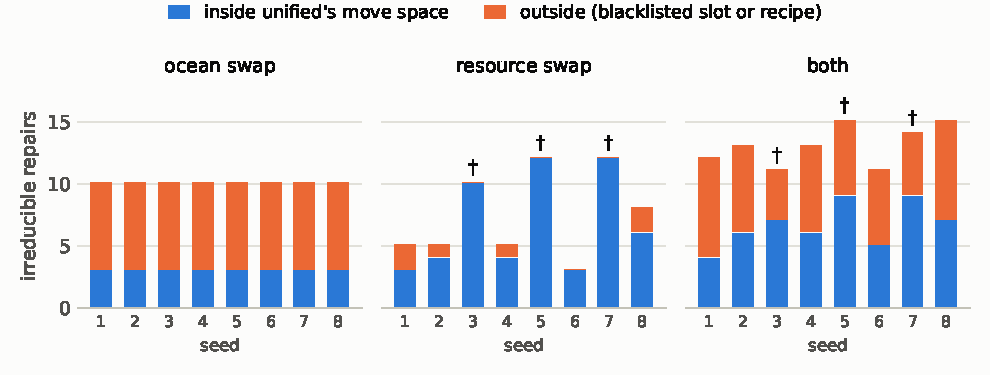
\includegraphics[width=\linewidth]{figs/where.pdf}
\caption{Irreducible repairs per seed (root-first order), split by whether unified's recipe-ingredients handler may randomize the slot. The ocean swap's repairs are the same on every seed, and 7 of its 10 are slots unified never touches. $\dagger$: the run also has goals that no ingredient repair can bring back (Vulcanus lost calcite), so its repairs are the leaf repairs that fix the rest.}
\label{fig:where}
\end{figure}

\begin{figure}[t]
\centering
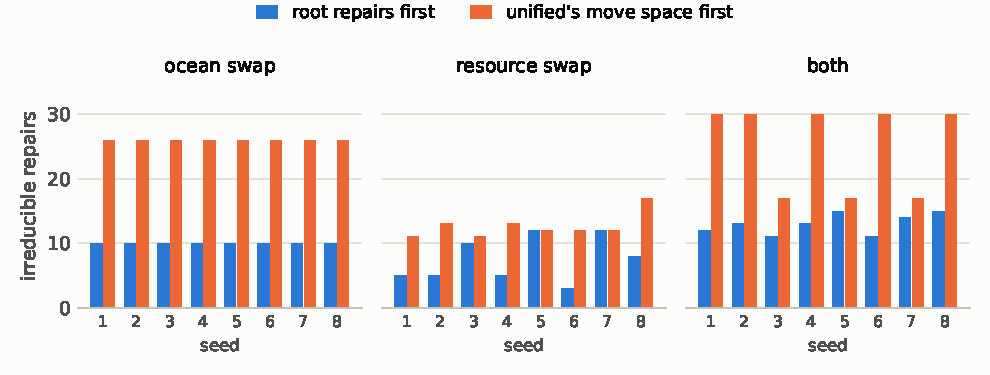
\includegraphics[width=\linewidth]{figs/uspace.pdf}
\caption{Irreducible repairs with root slots ordered first (blue) versus with unified's whole move space ordered first (orange), per seed. For the ocean swap, unified's move space needs 26 slot changes instead of 10 on every seed, because it can only reach the contradictions from the consumers' side. The gap nearly closes on seeds 3, 5 and 7, where Vulcanus loses calcite and the root-first order needs leaf repairs as well.}
\label{fig:uspace}
\end{figure}

\ResultsWhere

\subsection{Context conflicts: when a repair must be a duplicate}\label{sec:conflict}

A relaxed repair says where to change a recipe, not what to put there. A recipe has a single ingredient list, and it must work in every context the recipe keeps.

\begin{definition}[Context conflict]
For a slot of recipe $r$ with required contexts $C_r$, let $\mathcal{A}(c)$ be the set of materials established in context $c$ before $\peb{r}{c}$. The slot is in \emph{conflict} if $\bigcap_{c\in C_r}\mathcal{A}(c)=\emptyset$.
\end{definition}

\begin{proposition}\label{prop:conflict}
A conflicting slot cannot be repaired in place. Splitting $r$ into copies, one per group of contexts that share a filler, repairs it. A recipe whose vanilla contexts all lie in one room can conflict only between the ability variants of that room.
\end{proposition}

This is the precise version of the rule the planetary stage already follows: ``originals only ever used on that planet in vanilla are edited in place'', while the others keep a planned ``X (Planet)'' duplicate. The rule is conservative. A \emph{shared} recipe (made on several planets in vanilla) does not always conflict, since the new filler may be available wherever the recipe is required. That happens, for instance, when the other rooms only require the recipe without isolatability and can import the filler. So duplicates could be rarer than they are now. Figure~\ref{fig:conflict} illustrates the definition. \ResultsConflict

\begin{figure}[t]
\centering
\begin{tikzpicture}[x=1cm,y=1cm]
\draw[thick, cvan, fill=cvan!8] (0,0) ellipse (2.3 and 1.25);
\draw[thick, cshift, fill=cshift!8, fill opacity=0.7] (3.0,0) ellipse (2.3 and 1.25);
\node[font=\small, text=cvan] at (-0.6,1.55) {$\mathcal A(\text{Vulcanus}|11)$};
\node[font=\small, text=cshift!80!black] at (3.6,1.55) {$\mathcal A(\text{Nauvis}|01)$};
\node[font=\small] at (-1.1,0) {new fluid};
\node[font=\small] at (4.2,0) {water};
\node[font=\scriptsize, align=center] at (1.5,0) {common\\filler?};
\draw[-{Stealth}, thick, crep] (5.6,0) -- (6.9,0);
\node[lbl, text=crep, align=center] at (6.25,0.45) {empty\\$\Rightarrow$ split};
\node[andn, anchor=west] (r) at (7.1,0.6) {$r$ on Vulcanus: new fluid};
\node[andn, anchor=west] (r2) at (7.1,-0.6) {$r$ elsewhere: original};
\end{tikzpicture}
\caption{A context conflict. If no single filler is available before $r$ in every context $r$ must keep, an in-place edit breaks some context. Splitting $r$ per group of contexts (a planned duplicate) does not.}
\label{fig:conflict}
\end{figure}

\subsection{What this means for ``unified fixes the contradictions''}

\ResultsMeaning
